
\documentclass[main.tex]{subfiles}

\begin{document}

\chapter{Softening and finite elements}
\label{LEC:CohesiveZone}

\section{Effect of element size on the strain localization for linear softening law}

\begin{figure}
\centering
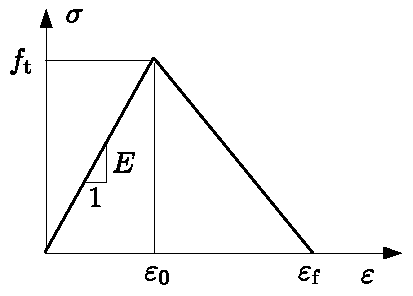
\includegraphics[width=6cm]{fig/Lecture08/fig_linear_softening}
\caption{Material with linear softening.}
\label{FIG_linear_softening}
\end{figure}

Instead of a cohesive crack model with the softening behavior described in terms of stress versus crack opening, let us consider a material law of a zone of a material with linear softening depicted in the Figure~\ref{FIG_linear_softening}. 
We will use the softening law to discretize a bar subjected to tensile load. The bar with the Young's modulus $E$ with the total length $L$ is discreitzed using $n$ number of elements.
The response of the bar will stay linear elastic until one of the elements reaches its tensile strength $f_\mathrm{t}$.
At this point, the strain in the bar will be $\varepsilon_0 = f_\mathrm{t} / E $. 
Thus, the elastic elongation of the bar can be expressed as
\begin{align}
u_\mathrm{el} = \varepsilon_0 L = \frac{f_t}{E} L
\end{align}
Beyond the elastic limit, the critical element will enter the softening branch while all the remaining elements will unload. Since we assume the linear softening behavior, we can directly obtain the nominal / macroscopic or average stress-strain response. Once the critical element reached the strength, the stress in the bar will decrease following either the unloading/elastic branch in the elastic part of the specimen or the softening branch in the single softening element. At the stress level $\sigma = 0$, the elastic part will unload to zero so that it provides no contribution to the overall displacement. The softening part will reach the strain corresponding to the intersection of the softening branch with the $\varepsilon$ axis, i.e. $\varepsilon_\mathrm{f}$. Thus, the control load upon reaching the zero strain in the bar be exactly
\begin{align}
u_\mathrm{f}  = \frac{L}{n}  \varepsilon_\mathrm{f}
\end{align}
As a result, the macroscopic stress-strain response of the bar is described by three data points for strains and stresses, i.e. 
\begin{align}
\varepsilon = [ 0, f_t/E, \varepsilon_f / n ], \sigma = [0, f_t, 0]
\end{align}
Apparently, the macroscopic response of the bar depends on the number of discretization elements so that we can produce arbitrary results by changing the number of elements or, more precisely, the size of the localizing element.

\begin{bmcsex}{Mesh bias for discretized bar with linear softening}{e81_discr_bar}
The example demonstrates that the bar response produces different results for 
different number of discretization elements.
See the example in \href{http://localhost:8888/tree/Examples/8.1 Mesh bias for discretized bar with linear softening.ipynb}{jupyter notebook}
\end{bmcsex}

% Remark: Characteristic length is a parameter calculated as
% \begin{align}
% l_{\mathrm{ch}} = \frac{E G_\mathrm{F}}{f^2_\mathrm{t}}
% \end{align}
% The intersect of the softening curve with the the -axis is given as $w_\mathrm{1} = \frac{G_\mathrm{F}}{f_\mathrm{t}}$


\section{Regularization of the softening law in finite element code}

Let us assume that the fracture energy $G_\mathrm{f}$ is known and  we want to improve the above model to deliver stable, mesh-independent results. Knowing that the energy dissipation is only happening in the one softening element, we can require that it alwas dissipates the same amount of energy. Recall that the fracture energy dissipated by a unit area of a stress free crack is evaluated as 
\begin{align}
G_\mathrm{f} = \int_0^{\infty} f(w) \, \mathrm{d}w
\end{align}
where $w$ represents the crack opening.
In the studied case of linear softening with $f$ defined as
\begin{align}
f(w) = f_\mathrm{t}\left( 1 - \frac{1}{w_\mathrm{f}} w \right)
\end{align}
and the corresponding fracture energy
\begin{align}
G_\mathrm{f} = \int_0^{w_\mathrm{f}} f(w) \, \mathrm{d}w = \frac{1}{2} f_\mathrm{t} w_\mathrm{f}
\end{align}
This kind of model is working correctly and reproduces exactly the amount of fracture energy needed to produce the unit area of the stress free crack. 

However, in a finite element model, the crack is not represented as a discrete line but is represented by a strain within the softening element of the size $L_s = L / N$. Thus, the softening is not related to crack opening displacement (COD) but to a strain in the softening zone using a softening function $\phi(\varepsilon_\mathrm{s})$. This model was used in the example above and delivered mesh-dependent results with varying amount of fracture energy.

To regularize the finite element model let us express the crack opening displacement as a product of the softening strain $\varepsilon_\mathrm{s}$ and the size of the softening zone $L_\mathrm{s}$:
\begin{align}
w = \varepsilon_\mathrm{s} L_\mathrm{s}
\end{align}
Now, the energy dissipated within the softening zone can be obtained as an integral over the history of the softening strain as
\begin{align}
G_\mathrm{f} = L_\mathrm{s} \int_0^{\infty} \phi(\varepsilon_\mathrm{s}) \, \mathrm{d}\varepsilon_\mathrm{s}
\end{align}
Comming back to the model with linear softening, the integral of the strain based softening function is expressed as
\begin{align}
\int_0^{\infty} \phi(\varepsilon_\mathrm{s})  \, \mathrm{d} \varepsilon_\mathrm{s} = \frac{1}{2} \varepsilon_\mathrm{f} f_\mathrm{t}
\end{align}
so that
\begin{align}
G_\mathrm{f} = \frac{1}{2} L_\mathrm{s} \varepsilon_\mathrm{f}
f_\mathrm{t}
\implies
\varepsilon_\mathrm{f} = \frac{2}{L_\mathrm{s}} \frac{G_\mathrm{f}}{ f_\mathrm{t}}
\end{align}

\begin{bmcsex}{Discretized bar with regularized linear softening}{e82_discr_bar}
This sheet provides the implementation of the above shown regularized softening model that does not change values for a modified size of the softening zone and delivers objective results.
See the example in \href{http://localhost:8888/tree/Examples/8.2 Regularized linear softening law for stable calculation in finite element code.ipynb}{jupyter notebook}
\end{bmcsex}

\section{Implementation of softening in finite-element codes}

Standard finite-elements are formulated for smooth shape functions and their derivatives within the element volume. Cracks in form of displacement jumps are not possible. Advanced finite-element techniques can be used to provide more accurate representation of strain localization of an emerging crack. These techniques, however, require changes in the mesh structure, remeshing, embedding of discontinuities or non-local integration of state variables including bookkeeping of neighboring relations between elements.  Implementation of these methods, however, is rather complex compared to standard finite-element methods so that these methods are rarely available in commercial codes and are mostly provided only in scientific codes.
 
In practical applications, the most common approach to introducing cracks is based on the concept of strain softening with smeared representation of a crack that resembles the approach studied in topic 7.2. This approach has been developed in the 1970’s and is used in the most commercial codes. In its original form the approach did not provide objective results and it was necessary to overcome a number of difficulties regarding the ill-posedness and lack of objectivity.

The common strategy applied in standard finite-element codes is the crack-band regularization technique. The basic idea of the crack band regularization is to relate the amount of energy dissipation to the size of the finite element. To illuminate the concept of crack band regularization, let us consider again the tensile test of a length  described in topic 7.2. The length of the softening element is .

We require that the energy needed to make the cohesive zone stress-free is equal to the energy required to produce a stress-free crack. More precisely: the amount of energy dissipated per unit area of an emerged crack must be equal to $G_\mathrm{F}$. Expressed mathematically, the softening law applied in a finite element computation with strain localization within a single finite element needs to fulfill the condition:
\begin{align}
G_\mathrm{F} = 
\int_0^\infty 
f(w) \; \mathrm{d}w
= 
\int_0^\infty 
\phi(\varepsilon) \; 
\mathrm{d} \varepsilon
\end{align}
This can be achieved by the requirement that the strain integral over the element exhibiting softening  is set equal to crack opening, i.e.
\begin{align}
w = \varepsilon h_c
\end{align}
where $h_c$ denotes the element length.  As a result, we can set
\begin{align}
\sigma = 
f_w(\varepsilon h_c) 
\end{align}

\section{Implementation of softening behavior in finite element code}

Consider a chain of 2 elements with the total length $L$. One element has slightly lower strength $f_t$. Then, upon softening we distinguish the elastic part of the length $L_\mathrm{el} = L (N-1)/N$  and the softening part with the length $L_\mathrm{s} =L/N$. The total elongation corresponding to the control displacement is then given as
\begin{align}
u = \varepsilon_\mathrm{el} L_\mathrm{el} + \varepsilon_\mathrm{s} L_\mathrm{s}.
\end{align}
The nominal/average strain in the whole bar can then be written as
\begin{align}
\varepsilon = \frac{\varepsilon_\mathrm{el} L_\mathrm{el} + \varepsilon_w L_w}{L}.
\end{align}
The stress in each of the two elements is
\begin{align}
\sigma_\mathrm{el} = E \varepsilon_\mathrm{el}
\end{align}
The equilibrium condition can then be written as a requirement of stress equality in both parts
\begin{align}
\label{eq:R:bar:equilibrium}
R = \sigma_\mathrm{el} - \sigma_\mathrm{s} = 0
\end{align}
The stress in the element $\mathrm{s}$ is governed by softening prescribed by the damage function
derived previously for a softening zone with predefined fracture energy in Eq.~(\ref{eq:damge_fn_fracture_base_exp})
\begin{align}
\omega(\varepsilon) =  
1 - \frac{f_t}{E \varepsilon} \exp(-\frac{f_t}{G_f} (\varepsilon - \varepsilon_0) L_s )
\end{align}
The resulting stress is provided as
\begin{align}
\sigma_\mathrm{s} = (1 - \omega) E \varepsilon
\end{align}
After substituting for stresses in Eq.~(\ref{eq:R:bar:equilibrium}) we obtain a residuum function as
\begin{align}
R = E \varepsilon_\mathrm{el} 
- 
( 1 - \omega(\varepsilon)) E \varepsilon_\mathrm{s} = 0
\end{align}
By using the compatibility equation we can express elastic strain in terms of the control displacement and softening strain as
\begin{align}
\varepsilon_\mathrm{el} =
\frac{1}{ L_\mathrm{el} }
\left( 
u - \varepsilon_\mathrm{s} L_\mathrm{s}
\right)
\end{align}
so that finally the residuum is given as
\begin{align}
R = \frac{1}{ L_\mathrm{el} }
\left(
u - \varepsilon_\mathrm{s} L_\mathrm{s}
\right)
 - (1 - \omega(\varepsilon_\mathrm{s}))  \varepsilon_\mathrm{s} = 0
\end{align}
This nonlinear equation can be solved iteratively using the Newton method. The first step is to use the Taylor expansion 
\begin{align}
\hat{R} = R(\varepsilon_\mathrm{s}^k) + 
\left.
\frac{ \partial R(\varepsilon_\mathrm{s}) }{ \partial \varepsilon_\mathrm{s} }
\right|_{\varepsilon_\mathrm{s}^k}
\Delta \varepsilon_\mathrm{s}
= 0
\end{align}
Using this approximation, we can calculate the increment of softening strain as
\begin{align}
\left.
\frac{ \partial R(\varepsilon_\mathrm{s}) }{ \partial \varepsilon_\mathrm{s} }
\right|_{\varepsilon_\mathrm{s}^k}
\Delta \varepsilon_\mathrm{s}
= 
-
R(\varepsilon_\mathrm{s}^k) 
\end{align}
The derivative of the residuum with respect to the softening strain reads
\begin{align}
\frac{ \partial R(\varepsilon_\mathrm{s}) }{ \partial \varepsilon_\mathrm{s} }
=
- 
\frac{L_\mathrm{s}} { L_\mathrm{el}} 
+
\frac{ \partial \omega(\varepsilon_\mathrm{s}) }{ \partial \varepsilon_\mathrm{s} }
\varepsilon_\mathrm{s}
- (1- \omega(\varepsilon_\mathrm{s}))
\end{align}
The iterative scheme is then given as
\begin{align}
\left[
- 
 \frac{L_\mathrm{s}} { L_\mathrm{el}} 
+
\left.
\frac{ \partial \omega(\varepsilon_w) }{ \partial \varepsilon_\mathrm{s} }
\right|_{\varepsilon_\mathrm{s}^k}
\varepsilon_\mathrm{s}^k
-
\left( 
1 - \omega(\varepsilon_\mathrm{s}^k)
\right )
\right] 
\Delta \varepsilon_\mathrm{s}
=
\frac{1}{ L_\mathrm{el} }
\left(
u - \varepsilon_\mathrm{s}^k L_\mathrm{s}
\right)
 - (1 - \omega(\varepsilon_\mathrm{s}))  \varepsilon_\mathrm{s}^k
\end{align}
The derivative of the damage function provided in Eq. (7).
\begin{align}
\frac{ \partial \omega(\varepsilon) }{\partial \varepsilon }
= \left\{ 
\begin{array}{ll}
0  &   \varepsilon \le \varepsilon_0 \\
\displaystyle{\frac{1}{E G_{\mathrm{F}} \varepsilon^{2}}}
f_{t} 
\exp \left({
- \displaystyle{\frac{L_\mathrm{s} (\varepsilon - \epsilon_{0})}{G_\mathrm{F}} f_{t}}} \right)
\left(G_\mathrm{F} + L_\mathrm{s} \varepsilon f_{t}\right)
 &  
\varepsilon > \varepsilon_0
\end{array}
\right.
\end{align}

\begin{bmcsex}{Iterative solution of the localization problem}{ex83_iterative}
The implementation of the described algorithm is provided in the notebook
It demonstrates the structure of a nonlinear finite element solver.
\end{bmcsex}

\mnote{Correspondence with the finite element code}
Derivation of this example follows the reasoning applied in the implementation of non-linear finite element computation. In the uni-axial case, we do not need to use numerical integration of stresses. The mapping between local strains and global strains, normally resolved using Jacobi transformation, is done by directly by multiplying the particular lengths. The notebook sheet supplied with the example increments the control displacement of the bar in an outer loop and searches for the solution satisfying the equilibrium condition in the inner loop.

\begin{bmcsex}{Standard finite element code}{ex74_tension_bar_localization}
When calculating this example using standard finite element code, the unknowns are the nodal displacements along the bar. Consider an example sketched in Figure~\ref{FIG_tension_bar}. It represents a bar with one element of a slighly lower strength $f_\mathrm{t}$ in a gray element then in the other elements. Upon displacement loading, the damage will localize in the gray element. The given geometrical and material parametric are preset in the BMCS application 
\texttt{Tensile test - isotropic damage}.

\paragraph{Tasks}
\begin{itemize}
\item Calculate the response using the jupyter script providedo in Example~\ref{ex83_iterative} and also using the BMCS application \texttt{Tensile test - isotropic damage}. Do they match?
\item Change the size of the softening zone to half and double size. Check to see if you get mesh-independent results.
\item Evaluate and plot the strain profile along the specimen with the three different sizes of the softening zone.
\item Compare the total amount of dissipated energy $G$ at the end of the loading with nearly zero force in the bar with the input value of the damage function $G_\mathrm{F}$. How are they related?
\item Switch off in the regularization using a button on the first page of the application. Then, the damage law is not adjusted to the element size any more. Change the size of the crack band element and test how does it affect the observed response.
\end{itemize}
\end{bmcsex}

\begin{figure}
\centering
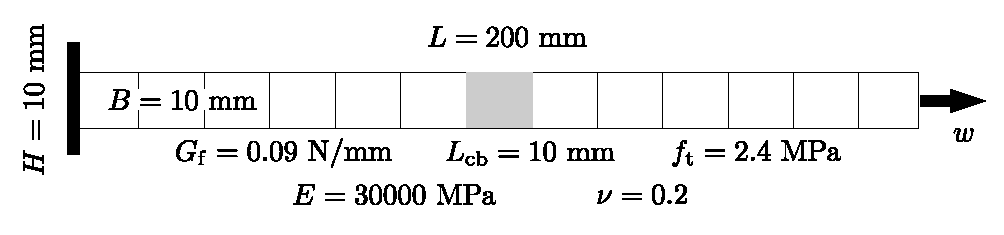
\includegraphics[width=12cm]{fig/Lecture09/figure_tension}
\caption{Example of a tension bar with a softening zone of a finite size.}
\label{FIG_tension_bar}
\end{figure}


\end{document}